%%%%%%%%%%%%%%%%%%%%%%%%%%%%%%%%%%%%%%%%%%%%%%%%%%%%%%%%%%%%%%%%%%%%%%%%%%%%%%%%
\documentclass[twocolumn]{revtex4}

%%%%%%%%%%%%%%%%%%%%%%%%%%%%%%%%%%%%%%%%%%%%%%%%%%%%%%%%%%%%%%%%%%%%%%%%%%%%%%%%
% Note that comments begin with a "%" and are not turned into text in the .pdf
% document.
%%%%%%%%%%%%%%%%%%%%%%%%%%%%%%%%%%%%%%%%%%%%%%%%%%%%%%%%%%%%%%%%%%%%%%%%%%%%%%%%

%%%%%%%%%%%%%%%%%%%%%%%%%%%%%%%%%%%%%%%%%%%%%%%%%%%%%%%%%%%%%%%%%%%%%%%%%%%%%%%%
% Include some extra packages.
%%%%%%%%%%%%%%%%%%%%%%%%%%%%%%%%%%%%%%%%%%%%%%%%%%%%%%%%%%%%%%%%%%%%%%%%%%%%%%%%
\usepackage[]{graphicx}
%%%%%%%%%%%%%%%%%%%%%%%%%%%%%%%%%%%%%%%%%%%%%%%%%%%%%%%%%%%%%%%%%%%%%%%%%%%%%%%%

%%%%%%%%%%%%%%%%%%%%%%%%%%%%%%%%%%%%%%%%%%%%%%%%%%%%%%%%%%%%%%%%%%%%%%%%%%%%%%%%
\begin{document}

%%%%%%%%%%%%%%%%%%%%%%%%%%%%%%%%%%%%%%%%%%%%%%%%%%%%%%%%%%%%%%%%%%%%%%%%%%%%%%%%
\title{
Final Project: Software Tools for Physicists 
}

\author{Taylor Muckle}
\affiliation{Siena College, Loudonville, NY}

\date{\today}

\begin{abstract}
    The goal of this final project was to determine whether or not a person could escape a velociraptor using our knowledge of physics, Python and LaTeX. The person was given a 30 meter head start before the velociraptor would start chasing them. The person's velocity was 3 m/s and the velociraptor's velocity was 18 m/s. After completing the following problems, the velociraptor caught up to the person after 2 seconds at 36 meters. The probability that a person could escape a velociraptor attack, with the given parameters, was about $67\%$.
\end{abstract}
\maketitle
%%%%%%%%%%%%%%%%%%%%%%%%%%%%%%%%%%%%%%%%%%%%%%%%%%%%%%%%%%%%%%%%%%%%%%%%%%%%%%%%
%%%%%%%%%%%%%%%%%%%%%%%%%%%%%%%%%%%%%%%%%%%%%%%%%%%%%%%%%%%%%%%%%%%%%%%%%%%%%%%%
\section{Problem #1}
Our goal in this problem was to plot the position versus time graphs for the velociraptor and person. We can start with the equation $x = xi + vi t + \frac{1}{2} a (t^2)$ and since we can ignore acceleration our new formula becomes $x = xi + vi t$. We can then make an equation using our known values for xi, vi and a range of values from 0-3 seconds for time. The velociraptor equation then becomes x = 0 m + (18 m/s)(t) and the person equation becomes x = 30 m + (3 m/s)(t).
To begin our plot, I imported numpy as np and matplotlib.pylab as plt. I then copied over matplotlib inline to make our graph appear in our notebook instead of on a separate page. I then labeled my x and y axes, gave my plot a title, and made appropriate window limits. Next, I imported the equations I made above and set a linspace line to make 1000 points on my graph from 0 to 3. Finally, I made a legend and chose my plot colors.
%%%%%%%%%%%%%%%%%%%%%%%%%%%%%%%%%%%%%%%%%%%%%%%%%%%%%%%%%%%%%%%%%%%%%%%%%%%%%%%%


%%%%%%%%%%%%%%%%%%%%%%%%%%%%%%%%%%%%%%%%%%%%%%%%%%%%%%%%%%%%%%%%%%%%%%%%%%%%%%%%
\section{Problem #2}

The goal of this problem was to figure out when the velociraptor caught up to the person and how far the person had run when that happened. To do this, I first calculated these values algebraically by setting my final position formulas equal to eachother, solving for time, and plugging the found time value in to find final position of the person. I found the time to be 2 seconds and the run position to be 6 meters. At first, I calculated 36 meters seemed to be a very large value until I realized that the person ran 6 meters but had a 30 meter head start.
For the coding part of the problem, I made a loop for going through my velociraptor and people speed formulas from time 0 to when they caught up. The goal is to get the formulas to give me the time at which they catch up and how far the person ran in that time. The loop says to tell me when the veociraptor equation equals the person equation, starting at 0; which gives the time 2 seconds, and the distance 6 meters(36-30).

\begin{figure}[b]
    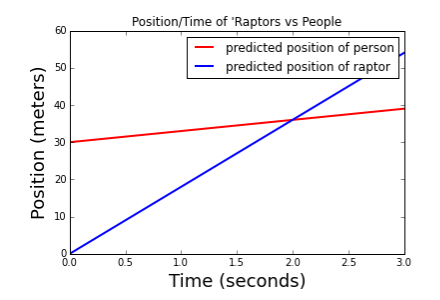
\includegraphics[width = 0.5\textwidth]{plot1_final.png}
    \centering
    \caption{This is my plot for comparing the velociraptor and people positions from times zero to three seconds. As seen in the plot, they catch up to each other at 2 seconds after the person has run 6 meters. \label{fig:Plot 1}}
\end{figure}

Check out the velociraptor and people positions in Fig.~\ref{fig:Plot 1}.

%%%%%%%%%%%%%%%%%%%%%%%%%%%%%%%%%%%%%%%%%%%%%%%%%%%%%%%%%%%%%%%%%%%%%%%%%%%%%%%%
\section{Problem #3}

The goal of this problem was to find when the velociraptor would strike and how far the person ran when they were attacked. The velociraptor would try to strike when it was one meter away from the person. I used the same set up as the previous problem, except this time I had to find the time and distance when the person and velociraptor were one meter apart. To do this, I changed my if statment to give me the time when the velociraptor was one meter behind the person by subtracting the person's distance by one at the time that it was one ahead of the velocirpator. I then used this time to give me the distance that the person was at. The time ended up being 1.888889 seconds at 35 meters; the person only ran 5 meters but had a 30 meter headstart. 
To make my plot, I remade the same plot as before and changed the colors. I then added and arrow showing the new time and distance I calculated.

\begin{figure}[b]
    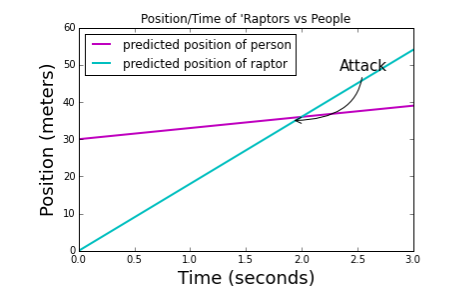
\includegraphics[width = 0.5\textwidth]{plot2_final.png}
    \centering
    \caption{This is my plot for comparing the velociraptor and people positions from times zero to three seconds. As seen in the plot, the person is one meter ahead at 1.888889 seconds after the person has run 5 meters. \label{fig:Plot 2}}
\end{figure}

Check out the velociraptor and people positions in Fig.~\ref{fig:Plot 2}.

%%%%%%%%%%%%%%%%%%%%%%%%%%%%%%%%%%%%%%%%%%%%%%%%%%%%%%%%%%%%%%%%%%%%%%%%%%%%%%%%
\section{Problem #4}

Our goal in this problem was to calculate the percent that a person could escape a velociraptor attack. We were told that "the first time it tries, there is a $20\%$ chance it will bite you. If it misses and it needs to try a second time, there is only a $15\%$ chance, and if it misses that time, there is only a $7\%$ chance on the third try. If it bites you once, you're 'raptor food. If it misses all three times, you get away!"
For my code, I decided to make nested conditionals for each trial the person edures. The first trial takes the number given by my random number generator (np.random.random(), which gives a random number between 0 and 1) and decides whether or not the number is less than $20\%$. If the number is less than that, the person dies and if not the move on to the next trial. The next trial is $15\%$ followed by $7\%$. If the person survives all three trials they get away from the velociraptor and if not they become snack.
I then ran my code a total of 30 times and found the average survival rate to be $67\%$.
%%%%%%%%%%%%%%%%%%%%%%%%%%%%%%%%%%%%%%%%%%%%%%%%%%%%%%%%%%%%%%%%%%%%%%%%%%%%%%%%
\end{document}
%%%%%%%%%%%%%%%%%%%%%%%%%%%%%%%%%%%%%%%%%%%%%%%%%%%%%%%%%%%%%%%%%%%%%%%%%%%%%%%%
